% !TEX root = paper.tex

\section {Results}
\label{sec:results}

\subsection{Ridge yield}

Figure~\ref{fig:PlotCorrMBHMT} shows two-particle correlation functions as functions of the relative pseudorapidity ($\Delta \eta$) and azimuthal angle ($\Delta \varphi$) differences between the trigger and associated particles. The functions are measured with Eq.~\ref{eq:corrfunction} for $1 < \pttrig~\mathrm{and}~\ptassoc < 2$ GeV/$c$ in pp collisions at $\sqrt{\it{s}} = $\unit{13} {\rm{}TeV}. The left figure is for the 0--0.1\% multiplicity class. The right one is from the minimum bias events (0--100\% multiplicity class). The ridge structure is clearly observed in the high multiplicity class compared to the minimum-bias events while no observation of the ridge in the minimum bias events. The away side is dominantly constructed by correlation of back to back jet.

\begin{figure}[h!]
	\centering
	\subfigure{ 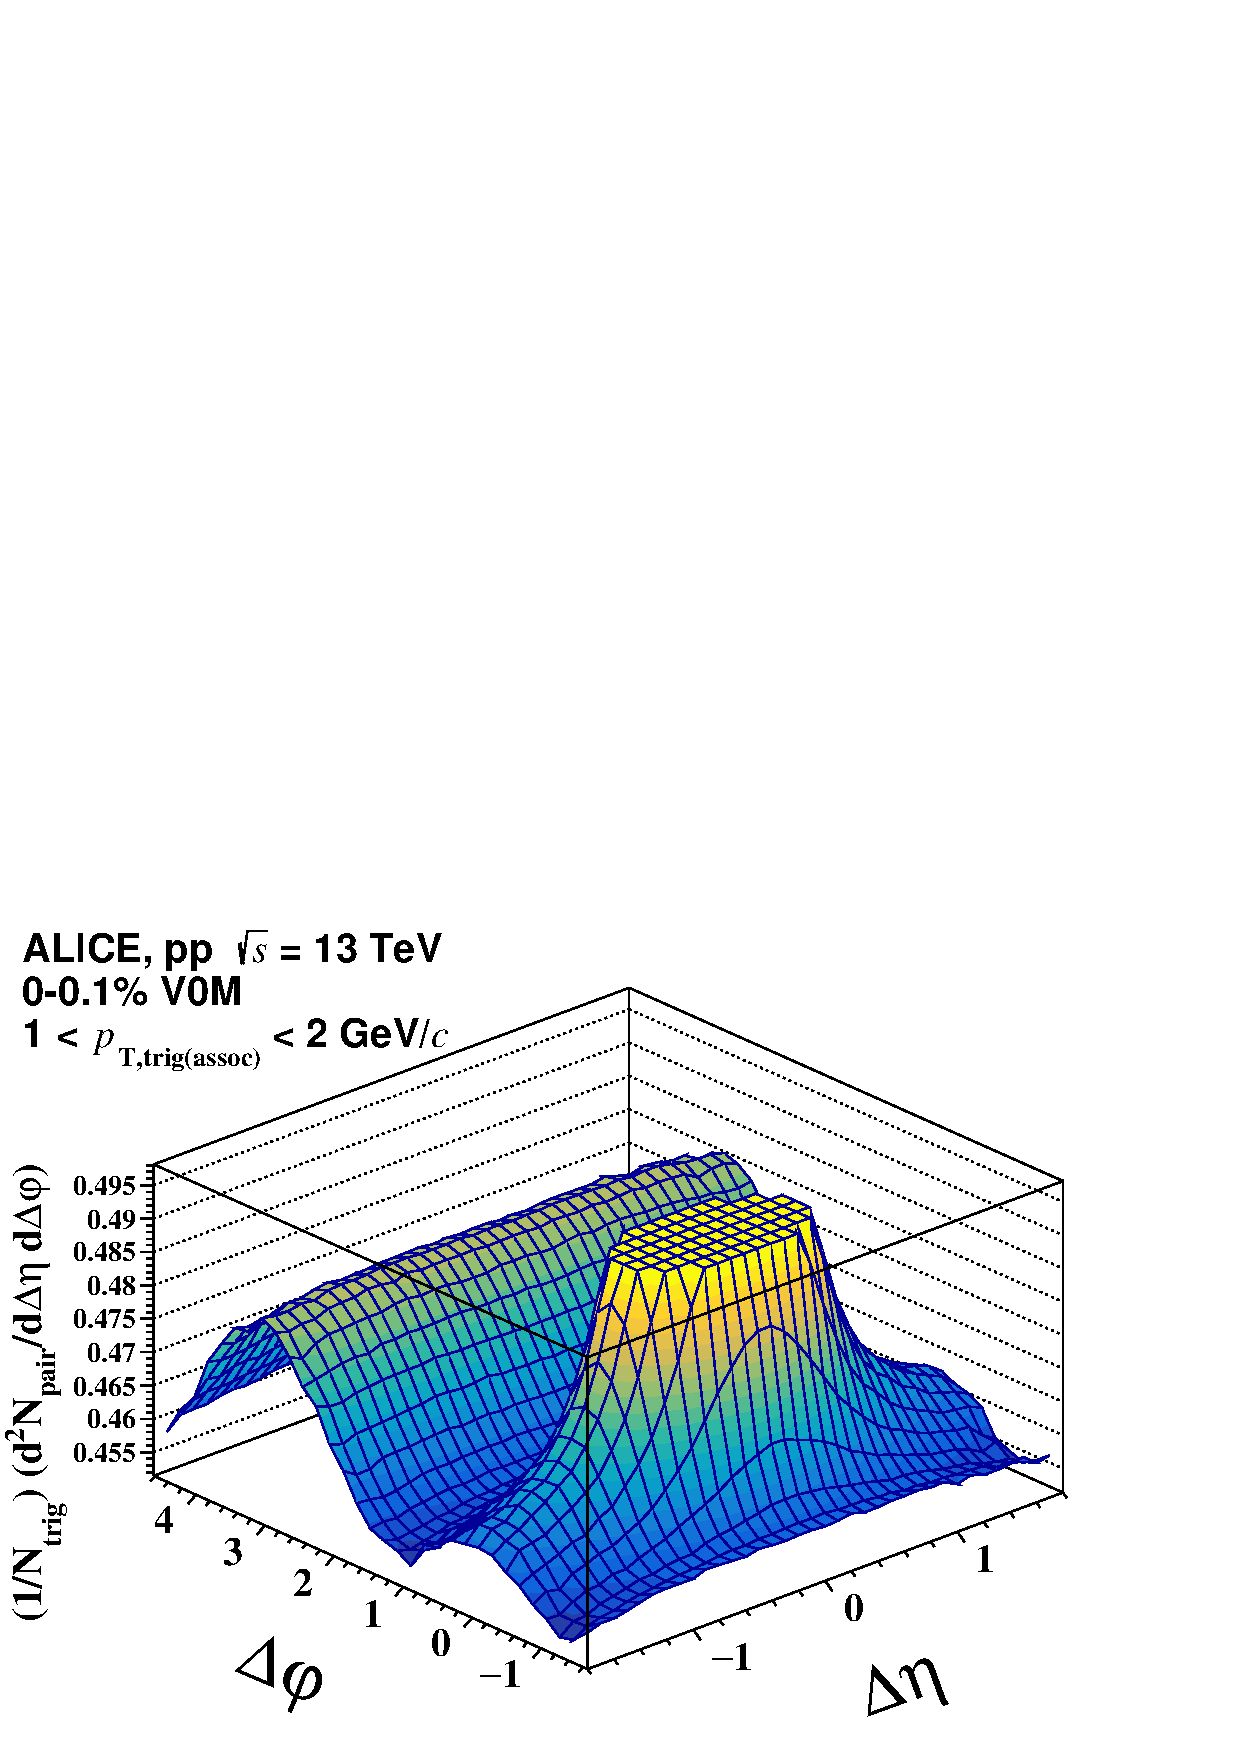
\includegraphics[width=0.47 \textwidth]{./figures/corr1.pdf} }
	\subfigure{ \includegraphics[width=0.47 \textwidth]{./figures/corrmb.pdf} }
	\caption{ Dihadron correlation functions as functions of $\Delta\eta$ and $\Delta\varphi$ in the high multiplicity (0--0.1\%, left) and the minimum-bias events (0--100\%, right). The intervals of $\pttrig$ and $\ptassoc$ are equally $1 < \it{p}_{\rm{T}} < 2$ GeV/$c$. }
	\label{fig:PlotCorrMBHMT}
\end{figure}

 Projected $\Delta\varphi$ distributions of the two-particle correlation functions in $1.6<|\Delta\eta|<1.8$ are shown in Fig.~\ref{fig:PlotDeltaPhi} for various $\it{p}_{\rm{T}}$ intervals in the high multiplicity class (0--0.1\%). The near-side peak is highest in the interval of $1<\it{p}_{\rm{T}}<2$ GeV/$c$ and gradually decreases with increasing $\it{p}_{\rm{T}}$.
 %The associated yield per trigger particle is compared with the CMS results. 


\begin{figure}[h!]
	\centering
	\includegraphics[width=0.99\linewidth]{./figures/Fig2_PlotDeltaPhi.pdf}
	\caption{One-dimensional $\Delta\varphi$ distribution in the large $\Delta\eta$ with various transverse momentum intervals in each multiplicity class. The distributions in upper panels are measured with 0--100\% multiplicity class. The distribution in lower panels are measured with 0-0.1\% multiplicity class. Interval of transverse momentum of trigger particle and associated particle is $1<\pt<2$ (left), $2<\pt<3$ (middle) and $3<\pt<4$ GeV/$c$ (right), respectively. }
	\label{fig:PlotDeltaPhi}
\end{figure}
 
The spectra of the ridge yield are shown in Fig.~\ref{fig:PlotYSpect} in the high multiplicity class and compared with the CMS results~\cite{Khachatryan:2015lva}. The estimator of particle multiplicity of ALICE is done with forward subsystem(V0), whereas that of CMS is done by mid-rapidity particles meeting with the condition of $|\eta|<$2.4 and $\pt>0.4$ GeV/$c$. Dedicated comparison is conducted and the difference of particle multiplicity is estimated to be about 20\%. Taking into account the difference in acceptance of charged tracks and comparable definition of multiplicity, the measurements are can be considered comparable with each other, which insists that measurements of azimuthal correlations can be achieved with ALICE. The spectrum is also compared with model predictions. $\pythiam$ and $\pythiashoving$ are used for the prediction. $\pythiam$ is shown with a black line and predicts no ridge effect in pp collisions, which is expected because the model does not implement any constraint to describe the ridge effect. $\pythiashoving$ shown with a red line describes the effect better than $\pythiam$, however, its yield decreases more rapidly than the data as $\pttrigassoc$ increases.

\begin{figure}[h!]
	\centering
	\subfigure{ \includegraphics[width=0.89\textwidth]{./figures/Fig3_PlotRidgeYield.pdf} }
	\caption{ The spectra of ridge yield as function of transverse momentum. The filled circles denote the measurement with ALICE and compared with CMS measurement~\cite{Khachatryan:2015lva}, which is represented as open box. The two lines show model predictions from $\pythiam$ (black line) and $\pythiashoving$ (red line). }
	\label{fig:PlotYSpect}
\end{figure}

\subsection{Event scale dependent ridge yield}

To further observe the behavior of the ridge yield with respect to the hard process, the correlation function is measured with the minimum $\ptlead$ (left) or $\ptjet$ (right) thresholds for $1<\pttrigassoc<2$ GeV/$c$, where the measured ridge yield is maximum in Fig.~\ref{fig:PlotCorrHMTSel}. The ridge structures are still seen with the event scale selection. With the minimum $\ptjet$ selection, the correlations function has a bump on the $\Delta\eta = 0$ and $\Delta\varphi = \pi$, which occurs due to the limited jet acceptance.

\begin{figure}[h!]
	\centering
	\subfigure{ 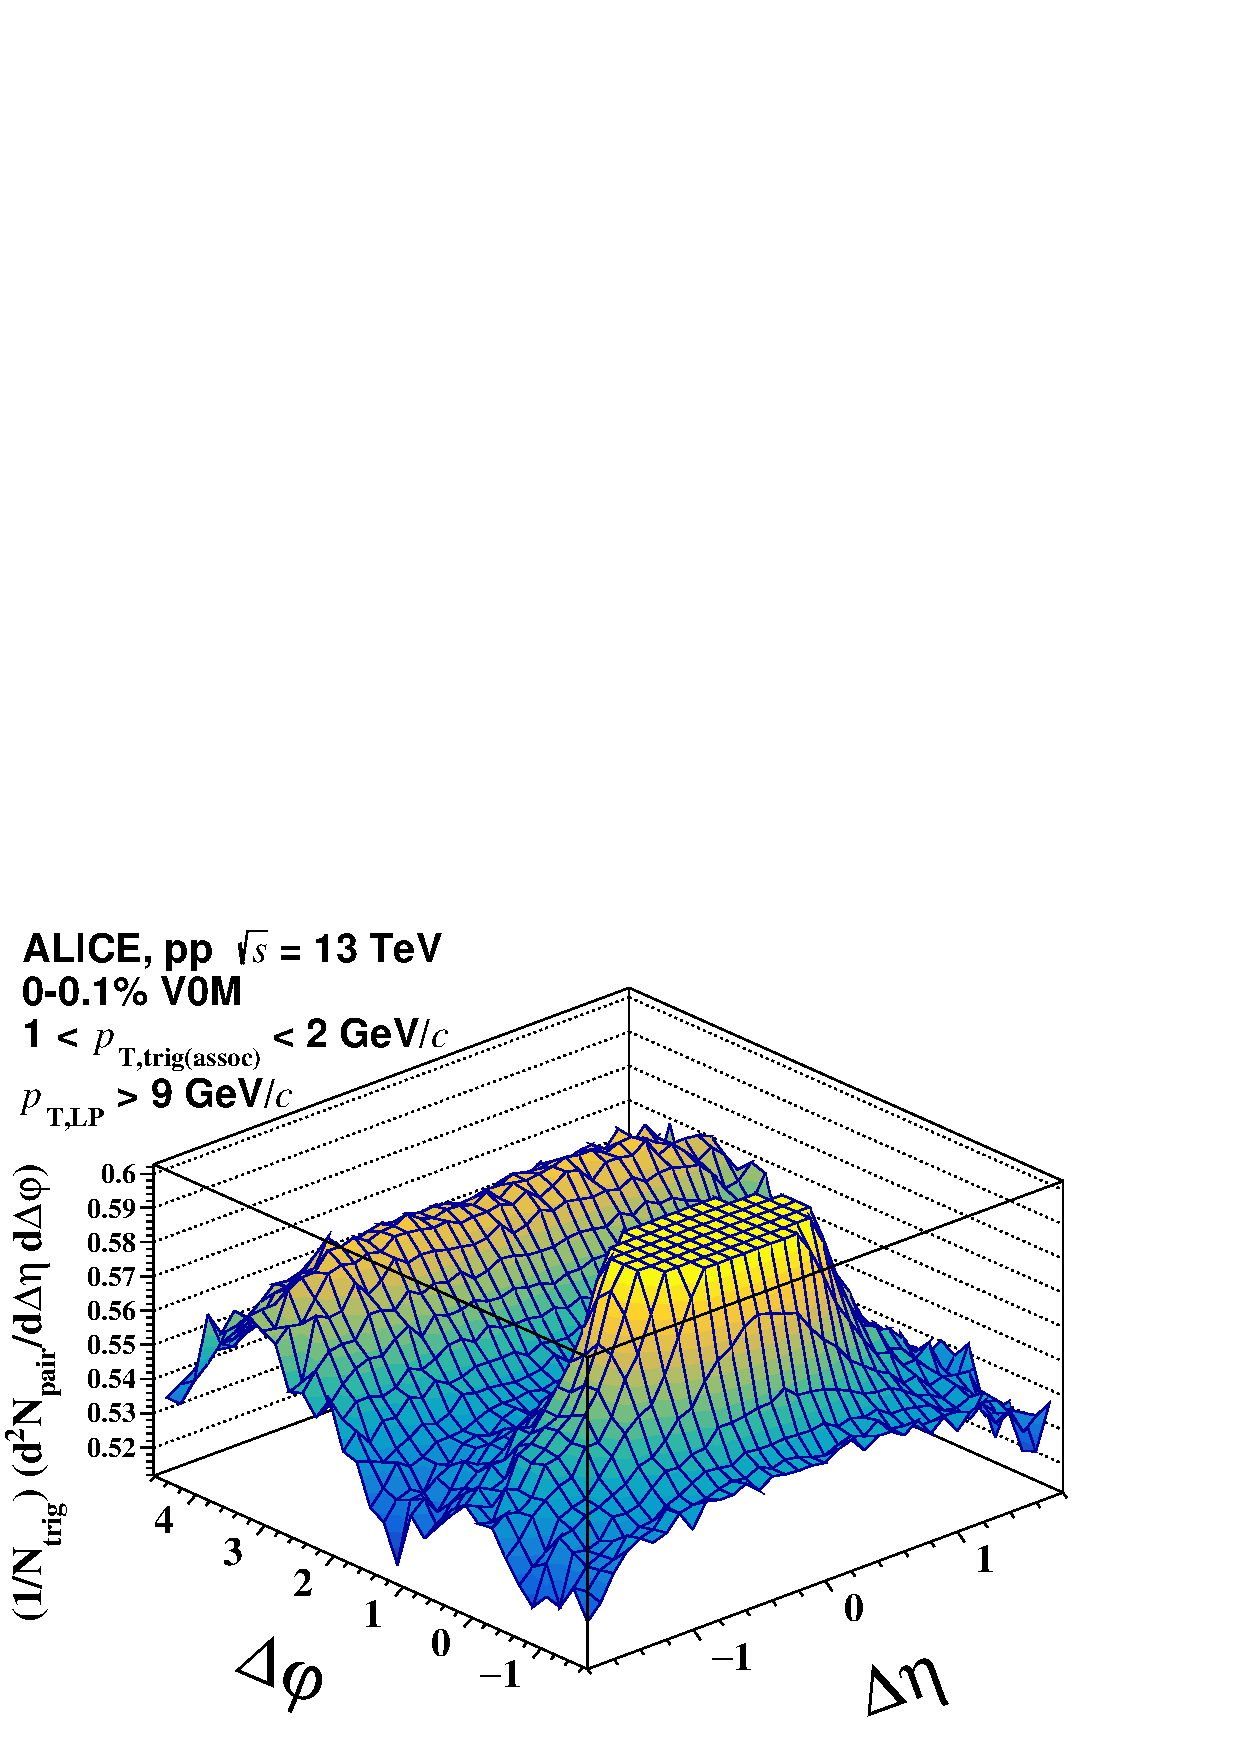
\includegraphics[width=0.47 \textwidth]{./figures/corrlh.pdf} }
	\subfigure{ 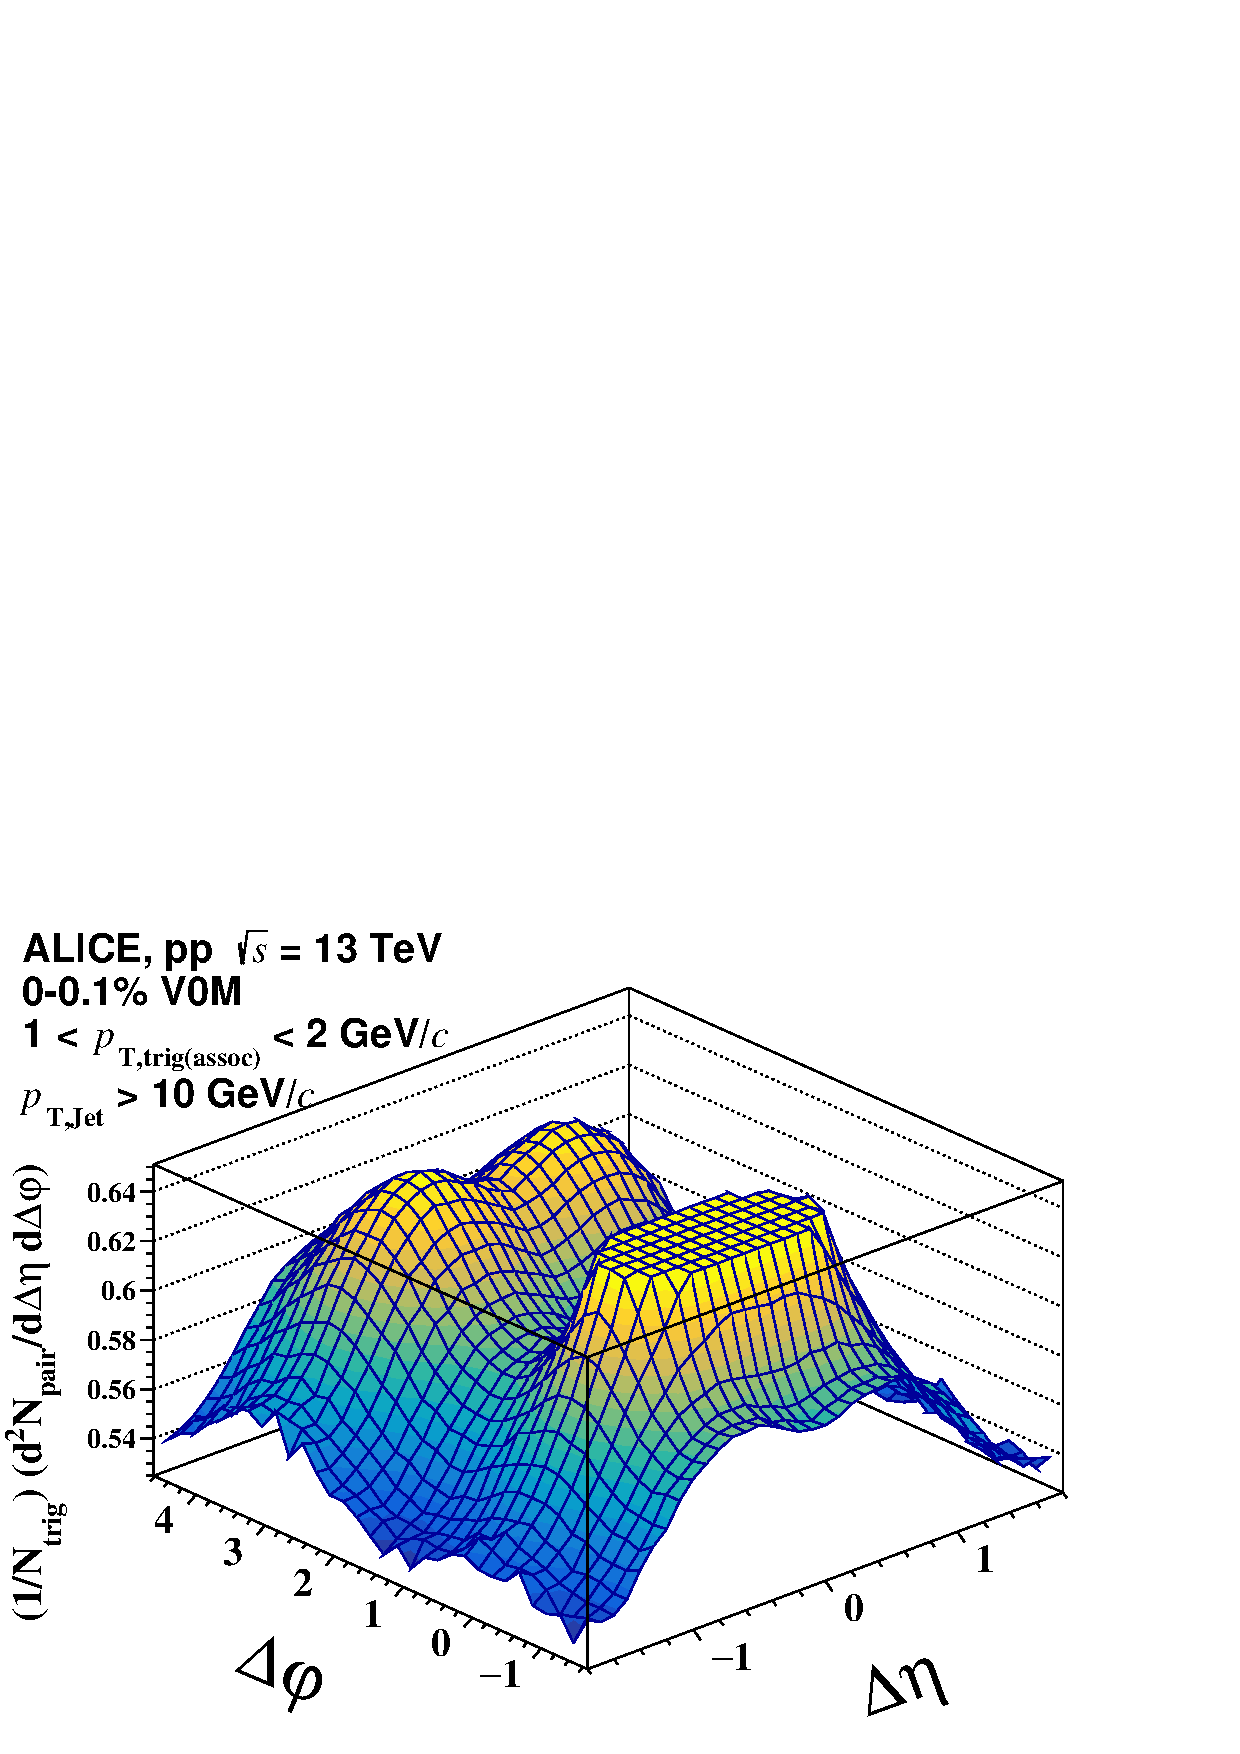
\includegraphics[width=0.47 \textwidth]{./figures/corrjet.pdf} }
	\caption{ Two-dimensional correlations function as function of $\Delta\eta$ and $\Delta\varphi$ in top 0-0.1\% multiplicity class with the minimum $\ptlead$ (left) or $\ptjet$ (right) selection. The interval of $\pttrig$ and $\ptassoc$ is $1<\pt<2$ GeV/$c$. The minimum requirement for $\ptlead$ or $\ptjet$ is 9 and 10 GeV/$c$, respectively. }
	\label{fig:PlotCorrHMTSel}
\end{figure}

The one-dimensional $\Delta\varphi$ distribution with the minimum $\ptlead$ (left) or $\ptjet$ is shown in Fig.~\ref{fig:PlotDeltaPhiESE}. The near-side yield increases as the event scale increases by requiring higher $\ptlead$ (left) or $\ptjet$. The model comparisons are are shown for $\pythiashoving$ with a blue and $\pythiam$ with a red line. The $\pythiashoving$ describes ridge yield with the selection. $\pythiam$ predicts non ridge yield with the selection, which also tell there is little ignore-able jet contamination. Both models well describe the away-side yield with the $\ptjet$ selection and overestimates away-side yield with the $\ptlead$ selection.

\begin{figure}[h!]
	\centering
	\includegraphics[width=0.99\linewidth]{./figures/Fig5_PlotDeltaPhiESE.pdf}
	\caption{ One-dimensional $\Delta\varphi$ distribution in the large $\Delta\eta$ with the minimum $\ptlead$(lower) or $\ptjet$(upper) selection for $1<\pttrigassoc<2$ GeV/\it{c}\rm{} in the 0--0.1\% multiplicity class. The filled circles show measurement with ALICE. Model predictions are compared with measurement with a blue line for $\pythiashoving$  and a orange line for $\pythiam$.}
	\label{fig:PlotDeltaPhiESE}
\end{figure}

The spectra of the ridge yield as function of the minimum $\it{p}_{\rm{T, Lead}}$(left) or $\it{p}_{\rm{T, Jet}}$(right) are shown in Fig.~\ref{fig:RidgeYield_ESE}. The spectra are compared with model predictions. 
The increases of ridge yield with the selections are observed and the model with PYTHIA8 + String Shoving underestimates the ridge yield. with the $\it{p}_{\rm{T, Jet}}$ selection. the model prediction with PYTHIA8 default still assures ignorable jet contamination.

\begin{figure}[h!]
	\centering
	\includegraphics[width=0.99\linewidth]{./figures/Fig6_RidgeYieldESE.pdf}
	\caption{The ridge yield spectra with respect to the leading particle and jet selections. The filled circles show measurement with ALICE. Model predictions are compared with measurement as blue line for PYTHIA8 + String Shoving  and apricot line for PYTHIA8 default.}
	\label{fig:RidgeYield_ESE}
\end{figure}



